\documentclass[thesis.tex]{subfiles}
\begin{document}
\chapter{Related Work}
\label{chap:related-work}

\section{Android and Mobile OSs}\label{android}
\todo{PUT IN THE DIFFERENCES BETWEEN THE SYSTEMS EXPRESSED IN APPPAL HERE AND MOVE IT TO CH4 WHEN DAVID TELLS YOU TO}

Android is a mobile operating system developed, primarily, by Google. It is by
far the most popular mobile operating system in use being installed on around
83\% of all mobile
handsets\footnote{\url{http://www.idc.com/prodserv/smartphone-os-market-share.jsp}}
with Apple's iOS being its only major competitor (Windows Phone, Blackberry OS
and other mobile operating systems account for only 3\% of the marketshare in
2015).

Despite the dominance of Android its ecosystem is rather fragmented. As shown in
Figure \url{fig:android-versions}, in June 2016 only 10\% of devices used the
latest version of Android, with around 5\% of devices still using a version
released five years prior. The range of different Android versions is often
blamed on the device manufacturers being unwilling to update their devices.
Since the core of Android is open source this has lead to third parties (such as
CyanogenMod\footnote{\url{http://www.cyanogenmod.org}}) have started developing
custom firmware for Android devices to allow older devices to be upgraded
independently of their manufacturers.

\begin{figure*}[htbp]
\centering
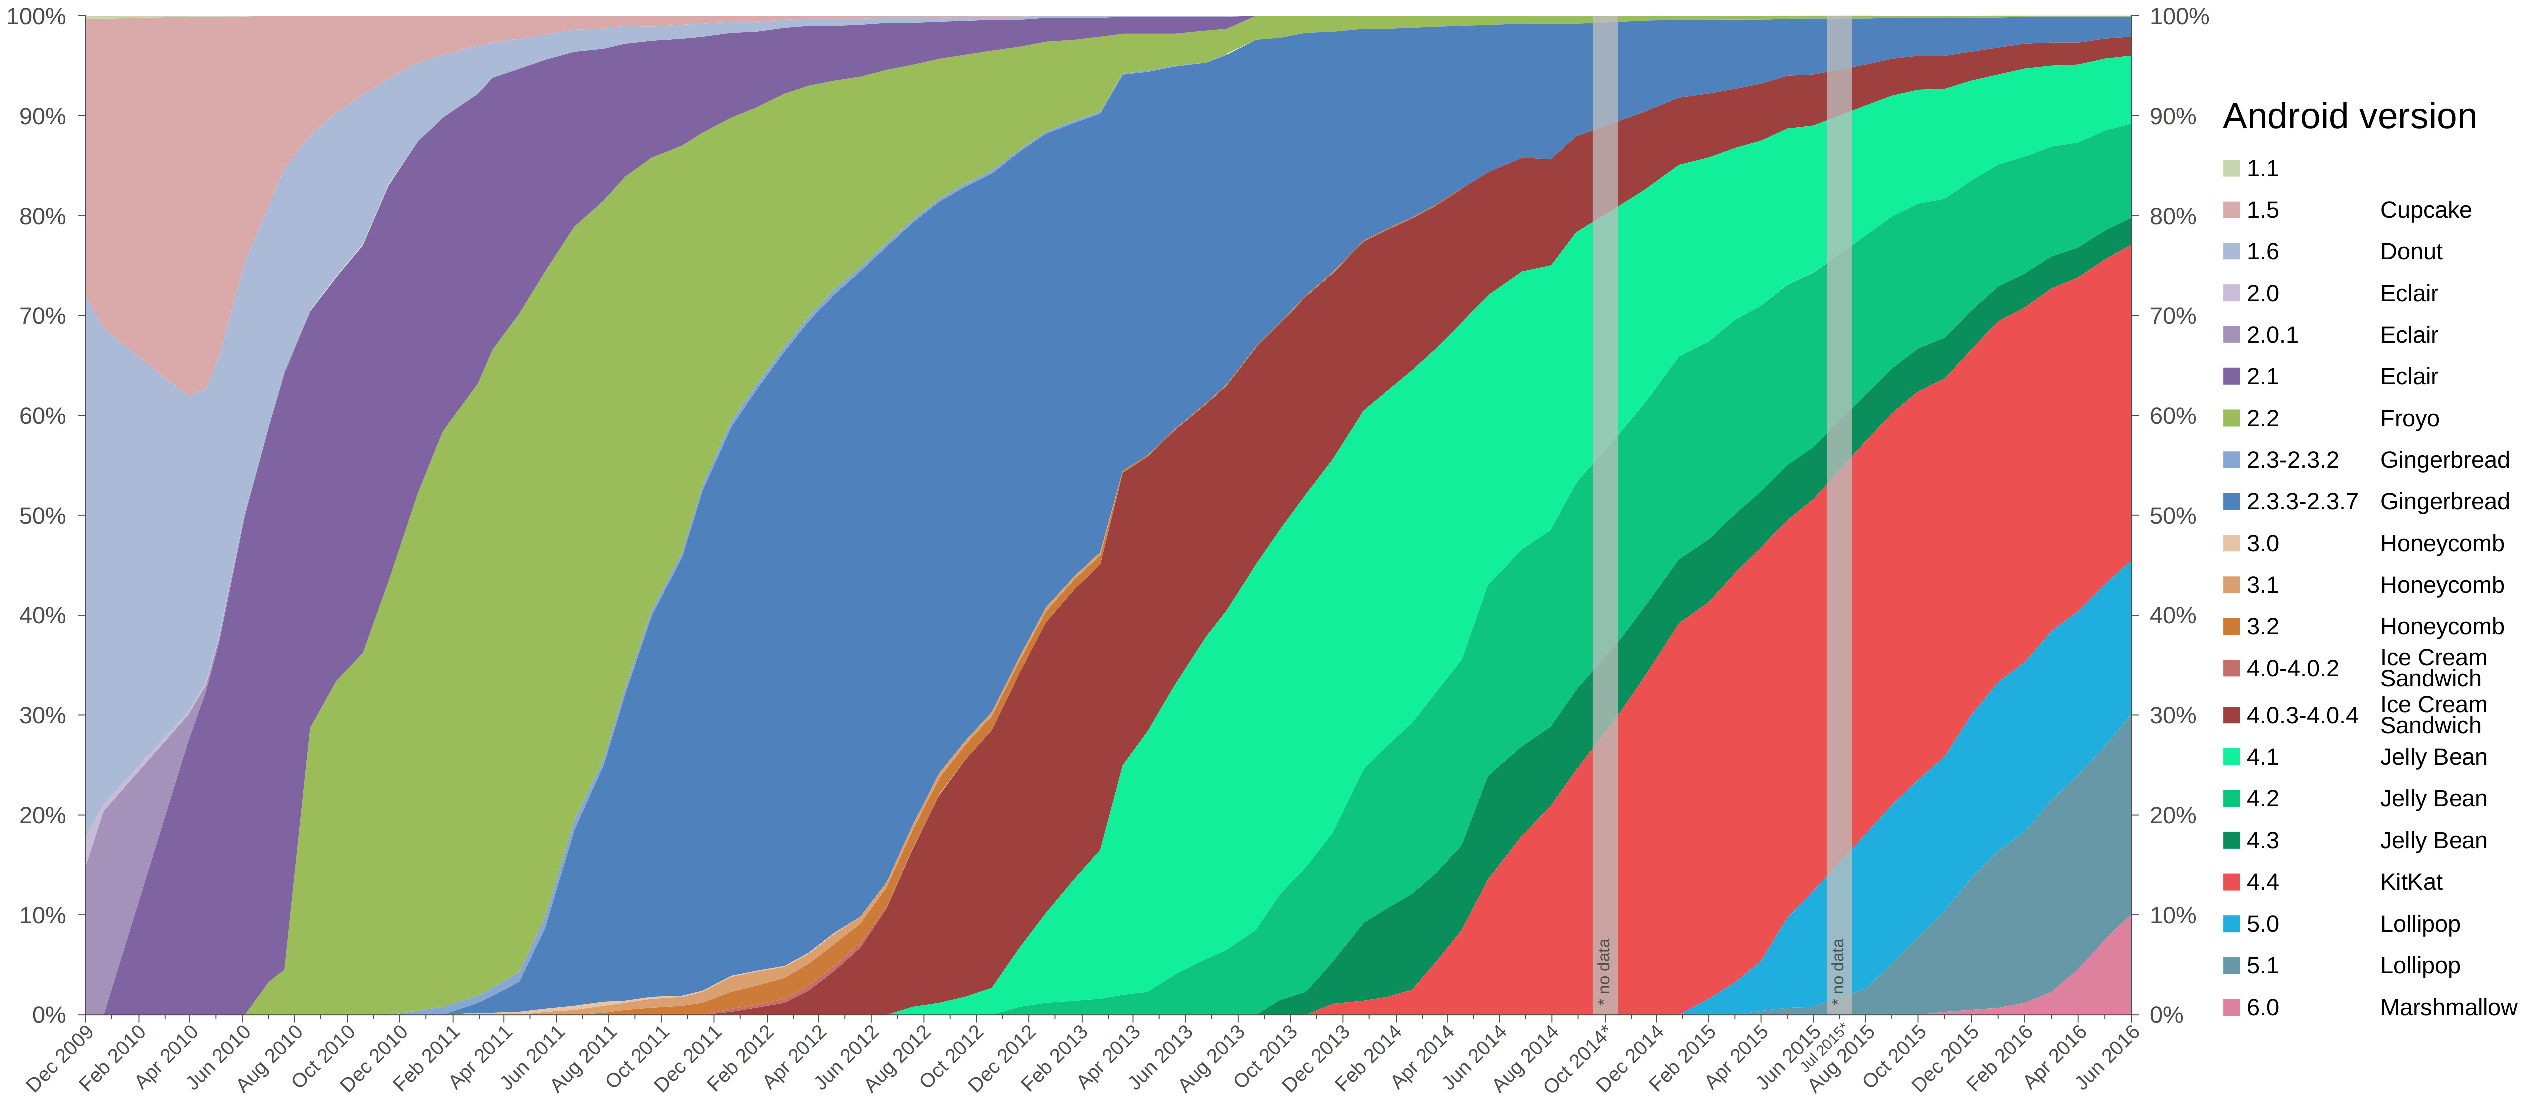
\includegraphics[width=\linewidth]{figures/android-versions.pdf}
\caption[Historical Android version's distribution.]{Historical Android
  version's distribution. Figure by \emph{Erikrespo} taken from
  \url{https://en.wikipedia.org/wiki/Android_version_history}.}
\end{figure*}

When building an Android device the manufacturers are also able to make
modifications to the Android firmware. This can be done to support any custom
hardware their device may have, add any additional software or apps, or provide
a custom look or theme to atheir device. Again this creates more variety in the
ecosystem, with few guarantees that any two devices may contain similar features
or hardware. In fact since the core of the Android is the Linux kernel (albeit
without the Linux Standard Base\footnote{The \emph{Linux Standard Base} is a
  specification produced by the Linux foundation that describes what a stardard
  Linux system should contain and how it should be organised. Android uses its own
  system which differs most noticably by the different filesystem structures and
  the use of user IDs to separate apps rather than users.
  \url{http://refspecs.linuxfoundation.org/lsb.shtml}}, and with additional
patches) it can be ported to other architectures (such as X86 and MIPS), and
used in other devices (such as set-top boxes and TVs, watches, and cars) with
relative ease.

To give developers a somewhat stable base to develop for Google developed the
\emph{Compatibility Test Suite}
(CTS)\footnote{\url{https://source.android.com/compatibility/cts/index.html}},
and \emph{Compatibility Definition Document}
(CDD)\footnote{\url{https://source.android.com/compatibility/android-cdd.html}}.
The CTS is a series of unit tests that check basic Android functionality and
behavior. The CDD is a document that describes what hardware an Android device
should have and how the device and it's software should be built. If a device
manufacturer wishes their device to run Google's Play Store (the largest Android
app marketplace), then they are required to show they can pass the CTS and are
in compliance with the CDD.

\section{Authorization Logic and Fine Grained Permission Systems}
\label{sec:authorization-logic}

\subsection{PolicyMaker and Keynote}
\subsection{SPKI/SDSI}
\subsection{RT}
\subsection{DKAL}
\subsection{Cassandra}
\subsection{XACML}

XACML is a standardised policy language~\cite{oasis_extensible_2013} that can be
extended to fit many scenarios. It is an attribute based policy language, but
can also describe role-based policies; and has industrial support from
\emph{Oracle}. XACML policies are expressed as sets of \emph{rules} that
describe whether a specific action should be allowed or denied. When making a
\emph{request} if a rule's target matches the request then the appropriate
action should be taken. Rules are combined into policies and may contain many
rules which can contradict each other if multiple ones match a given request. To
handle contraditions between rules a \emph{combining algorithm} may be used to
decide how to proceed. Typical algorithms include:

\begin{description}
  \item[Permit-overrides] where if a single rule gives a permit result then the request is permitted.
  \item[Deny-overrides] where if a single rule gives a deny result then then the request is denied.
  \item[First-applicable] where the rules are given an order of precedence and the first rule in the order that gives a result decides the outcome.
  \item[Only-one-applicable] where only one rule may match, and if there are multiple matches an error is returned.
\end{description}

XACML is a powerful access control and policy language with a published
standard~\cite{oasis_extensible_2013}. It is generic and is used in industry as
a policy language for access control decisions, and there are tools available to
help policy authors write policies in it. Whilst XACML might seem like a
suitable language to model mobile ecosystems, it suffers from various issues.

Readability was a design goal for SecPAL. Its notation is similar to natural
language. Alternate notations based on XML do exist (Becker hints at them in the
SecPAL technical report~\cite{becker_secpal:_2010}); though these are to aid
computerised parsing of SecPAL not human legibility. In contrast, XACML's
default syntax is difficult to read. XACML policies are verbose, and written in
XML. To help developers write policies alternative notations are available that
compile into XACML's XML notation. ALFA is an alternate notation for
XACML~\cite{oasis_xacml_technical_comitee_abbreviated_????}. The XACML
developers maintain ALFA, however others notations exist including graphical
languages~\cite{henrik_nergaard_scratch-based_2015}, languages based on
propositional logic~\cite{zhang_synthesising_2004} and answer set
programming~\cite{ramli_xacml_2012}.

\todo{MORE DETAIL EMPHASISE SEMANTIC PROBLEMS}
XACML does not have well-defined semantics. XACML's designers used natural
language to describe the semantics of XACML. This has made the semantics
notoriously difficult to interpret~\cite{ramli_detecting_2015}. There have been
several attempts to describe XACML's semantics
formally~\cite{ramli_xacml_2012,ramli_logic_2014,bryans_reasoning_2005}. These
help specify XACML but the lack of a single standard semantics make it less
attractive to extend to a new domain. In contrast, SecPAL's semantics are given
precisely by Becker~\cite{becker_secpal:_2010}

Whilst XACML 3.0 does support delegation~\cite{oasis_xacml_2010}, earlier
versions do not. The XACML 3.0 standard was published in 2013, after deciding to
start work with SecPAL.

\todo{GIVE EXAMPLES OF XACMLS SYNTAX}

\subsection{Dr.~Android and Mr.~Hide}
\subsection{Aurasium}
\subsection{CRePE}
\subsection{Kirin}
\subsection{SEAndroid}

\section{Static analysis tools}

There have been many static tools developed that can infer complex
properties about
apps~\cite{felt_android_2011,song_integrated_2016,antonin_carette_investigating_2017,schmidt_static_2009,enck_taintdroid:_2014}.
Leveraging these tools in a policy language lets us make statements about the
properties they can infer, without having to reimplement the functionality.
Despite the power of these tools it is not obvious how they should integrate
with the policies surrounding the mobile ecosystem. Running and configuring each
It isn't clear when each tool should run, or how to configure them to enforce a
policy rule. By incorporating these tools into a policy language, such as
SecPAL, we can act as a glue-layer between the policies of the mobile ecosystem
and the research into the properties of code.

\end{document}

%%% Local Variables:
%%% mode: latex
%%% TeX-master: "../ch7.tex"
%%% End:
